\chapter{Post-GWAS: where next? More samples, more SNPs or more biology? \cite{marjoram14}}
\label{cha:research_topic_3}

\section{Introduction}
We live in the era of genome-wide association studies (GWAS), a time in which vast efforts have been made to find single-nucleotide polymorphisms (SNPs) that are associated with phenotypic variation. This has led to the discovery of a large number of associated SNPs— 1617 published GWAS `hits' at $P < 5 \textsc{x} 10^{-8}$ for 249 traits as of the third quarter of 2011, the latest figures available from http:// www.genome.gov. However, there is a growing awareness that the majority of phenotypic variance apparently remains unaccounted for. This has led to a search for this missing heritability (for example, \cite{Manolio2009, Eichler2010} ).

There are at least two possible explanations for missing heritability. First, it may be a consequence of our inability to interrogate all SNPs in a region using so-called SNP-chip array platforms. This has led to a growing enthusiasm for the use of next-generation sequencing technologies with which, in principle at least, all polymorphism in a region can be discovered. However, another possible explanation for missing heritability is that we are not performing the correct analysis of the data we are collecting or we are not estimating heritability in the correct way \cite{Zuk2012}. GWAS typically looks for simple, marginal effects of SNPs on phenotypic variation. However, disease is often complex. As an example, Zuk et al. \cite{Zuk2012} illustrate how simple, nonlinear models can lead to phantom heritability. It is possible (and we believe likely to be) that analyses that move beyond agnostic, marginal tests of association will lead to the amount of missing heritability being significantly reduced. With this in mind, we briefly overview three interconnected pillars of assumptions, which serve as foundations for the marginal GWAS approach: (i) additive genetic variation is abundant, (ii) individual causal polymorphisms have sizable effects and (iii) those polymorphisms segregate at moderate-to-intermediate frequencies. Arguably, a fire has recently begun smoldering under each of these three pillars. We will focus on the brightest flames illuminating the limitations of the traditional GWAS approach. As is frequently the case, these same flames also cast light on possible future directions. Thus, we end on optimistic notes sounded by clues present in recent research.

We begin by discussing each of the three pillars in turn:

\subsection{Pillar 1: Additive genetic variation is abundant}

For decades, programs of stock improvement have relied on the breeders' equation, based on resemblance between relatives \cite{Lynch1998}. These programs have been tremendously successful, resulting in productivity increases of several folds \cite{Falconer1996}. However, the reason why the breeders' equation works remains a subject of debate (and, of course, the plant breeding community has made much progress without it). The problem is that phenotypes arise from principally nonlinear molecular biological processes underlying developmental, signaling and metabolic cascades. Is the additive component of genetic variation, in fact, predominant? Hill et al. \cite{Hill2008} became so alarmed by this issue that they reanalyzed an impressive array of data. They overwhelmingly confirm widespread additivity. They hypothesized that a population genetic process referred to as mutation-selection balance may result in patterns of segregation in casual polymorphisms in which the variation will appear additive even though the pathways through which the phenotypes are affected are highly nonlinear. Indeed, mutation-selection balance can account for most, though hardly all \cite{Houle1998}, of the genetic variation in phenotypes. Under mutation-selection balance most mutations segregating in a population are partially recessive, and they are present at low frequency. Hill et al. \cite{Hill2008} show that under these conditions, most variation will appear additive irrespective of the architecture of the molecular network.

Gjuvsland et al. \cite{Gjuvsland2011} have approached the issue from a different angle, basing their considerations not in population genetics but in network architecture principles. Indeed, population genetics might represent a somewhat shaky foundation upon which to build. If mutations do not contribute to additive variation, natural selection to keep them at low frequency might be ineffective \cite{Charlesworth1996}. If additive variation is removed but non-additive variation accumulates, the outcome might be envisioned as predominantly non-additive variation. Gjuvsland et al. \cite{Gjuvsland2011} show that, in populations with intermediate allele frequencies, randomly generated genotype–phenotype (GP) maps generate proportions of additive heritable variation ($V_a$), among overall variation due to segregating polymorphisms ($V_g$), that are far lower than is empirically observed. They, therefore, argue that the special nature of molecular networks might lead to additivity, even though the networks themselves are nonlinear. As an example of this, they consider the property of `order-preservation', in which the network architecture prevents `order- breaking' \cite{Gjuvsland2011}.

Although both explanations are elegant and intuitive, they in no sense represent a final answer. Indeed, they present particular cases in which $V_a$ would be the main component of variation but they do it by imposing constraints (on the frequency of causal mutations or on network architecture) that do not have to be generally correct. Zuk et al. \cite{Zuk2012} approach the same problem from a different angle. They again start from the common observation that causal polymorphisms detected in GWAS on tens of thousands of individuals appear to account for only a small fraction of heritable variation for a given complex disease. They argue that this conclusion is often drawn because investigators typically, and mistakenly, equate narrow sense heritability, $V_a$, with the estimate of heritability resulting from pedigree studies, $V_g$, which includes effects due to epistasis. This results in a concept they term `phantom heritability'. When compared with $V_g$, much heritability appears to be missing; but when compared (correctly) with $V_a$, much of the missing heritability disappears. Using an example of a particular nonlinear network, they present simulations showing that only a fraction of heritable variation need be truly additive. In such a context, if causal polymorphisms are found as contributing to that truly additive component (rather than highly inflated pedigree-based estimates), the polymorphisms identified would have accounted for most–if not all–of $V_a$. Thus, from their perspective the problem of `missing heritability' should be re-termed as a problem of `inflated $V_a$ estimates'. For a nice overview of issues related to heritability in the GWAS era, see Zaitlen and Kraft (2012)\cite{Zaitlen2012}.

Building on the helpful framework provided by theoretical analyses such as those discussed above, one possible way forward is to analyze genetic variation in the networks directly, observing whether linear models account for a significant fraction of natural variation. We have implemented this approach for sex determination \cite{Tarone2005}, and InR/TOR \cite{Nuzhdin2009} pathways in flies. We proposed \cite{Tarone2012} that small-effect mutations might be well approximated by linearization around steady flow in nonlinear pathways. Whether and to what extent this explanation is generally correct is fertile ground for future research.

\subsection{Pillar 2: Individual causal polymorphisms have sizeable effects}

Inferring causal polymorphisms that account for, but, a tiny fraction of quantitative variation would require an enormous sample size \cite{Long1999}. The sizes of GWAS studies are now reaching multiple thousands of individuals, in part, due to a move toward meta-analysis in recognition of the consequent power benefits (for example, \cite{Lindgren2009,Stahl2010}). However, causal polymorphisms can only be reliably detected if they account for a sizable fraction – on the order of 1\% - of phenotypic variation \cite{Long1999}. Is it reasonable to hope that most polymorphisms have such large effects? The literature on this topic is nearly overwhelming and we are able to cover only a few highlights here. At the beginning of the QTL era, arguments that phenotype would typically be explained by a few loci of major effect were abundant (for example, \cite{Mackay2001}). It was fast realized, however, that the effect sizes are typically overestimated - the so-called Beavis effect (Beavis, 1994). The problem is that the lower the power of an assay, the greater is the resulting overestimation of effect size \cite{Lynch1998}. This is related to the effect known as the `Winner's Curse' in the GWAS field, in which it was also noted that effect sizes for significantly associated loci will typically be overestimated \cite{Kraft2008}.

Is it possible to `back-calculate' the true distribution of the effect size of causal polymorphisms given their estimated effect sizes? Otto and Jones \cite{Otto2000} showed that it is possible to estimate the total number of associated loci from such data, but did not address bias correction. The emerging best practice to avoid the Winner's Curse is to infer the set of causal polymorphisms in one population, whereas estimating their effects in a different, fully independent population \cite{Kruglyak2008}. Although utilizing data from several populations has become a common practice in yeast and human studies, other models do not afford similar replication. In conclusion, the distribution of effect sizes contributing to standing quantitative variation remains unclear.

As an illustration of this in a series of recent manuscripts, Mackay et al. \cite{Mackay2012}, Jordan et al. \cite{Jordan2012} and Weber et al. \cite{Weber2012} identified a relatively small number of candidate polymorphisms that might account for the majority of phenotypic variation. The analytical approaches used rest on the underlying assumption that a few major polymorphisms matter; the conclusions support this conjecture. Alternatively, Ober et al. \cite{Ober2012} reanalyzed some of the same data under a different assumption—the `nearly infinitesimal' model - that assumes numerous polymorphisms, each with rather small effect size. In this paper, they calculate genetic relatedness among genotypes, compare it with phenotypic resemblance and calculate the fraction of phenotypic variation accounted for. The conclusion was that on the order of 8\% of phenotypic variation is explained, consistent with the expectation for the experiment sample size. Overall, genetic polymorphisms appear to have accounted for modest amounts of variation. We stress that the two above analyses, made under diametrically opposed assumptions, resulted in rather divergent conclusions. This is unsurprising as the truth probably represents a mix of larger and smaller effect mutations, and the analyses above pick from opposite tail of this distribution. There has been additional recent progress in this area using models mixing both assumptions in the context of variance component or mixed models \cite{Kang2010, Korte2012}. However, a general picture is yet to emerge.

\subsection{Pillar 3: Individual causal polymorphisms segregate at moderate-to-intermediate frequencies}

The debate over `common mutation - common disease' versus `rare mutations - common disease' models has proven to be the source of a great number of manuscripts, including many recent reviews (for example, \cite{Manolio2009}). We raise this issue only insofar as it relates to the prospect for GWAS. Recall Hill et al. \cite{Hill2008}. If causal polymorphisms are at low frequency, they contribute to additive variation. However, the power to detect such polymorphisms is rather low, potentially requiring prohibitive sample sizes \cite{Zuk2012}. Curiously, as power drops with allele frequency, the resulting expected overestimation of effect size increases \cite{Lynch1998}. Accordingly, less frequent causal polymorphisms will appear to have a stronger effect than is actually the case \cite{Mackay2012}, perhaps biasing the flow of resources from GWAS to the `mutational screen' paradigms that have recently been gaining in popularity \cite{Tennessen2012}.

What proportion of phenotypic variation is, then, due to low-frequency (as compared with intermediate frequency) alleles? Referring back to Mackay et al. \cite{Mackay2012}, Jordan et al. \cite{Jordan2012} and Weber et al. \cite{Weber2012}, low-frequency mutations matter. This is problematic for GWAS if effect sizes are relatively small. However, per the analysis of Ober et al. \cite{Ober2012}, the intermediate frequency alleles matter. This in itself may pose problems for GWAS analyses that focus on detecting additive effects since, as discussed above, although apparent additivity is likely to be for rare variants, it is not a necessary consequence for alleles of intermediate frequency.

To summarize, GWAS will be most successful, if (i) additive genetic variation is abundant, (ii) individual causal polymorphisms have sizable effects and (iii) they segregate at moderate-to-intermediate frequencies. So, is genetic variation mostly additive? In general, we do not know. Do individual causal polymorphisms have sizable effects? Again, in general we do not know. Do they segregate at moderate-to- intermediate frequencies? Once again, we do not really know. Overall, it appears that we are still some way short of certainty in affirming these requirements, at least in the Drosophila model we feature in this chapter.

\section{The way forward: `Post GWAS'}
From the preceding discussion, it is tempting to generalize that the answer ‘we do not know’ is the only ‘true answer’ and the minute one claims that he ‘knows’, he is wrong \cite{Pelevin2001}. This response is obviously unsatisfactory, particularly if it might undermine a paradigm, which is seen as a significant step toward future advances in health and agriculture. Alternatively, might the GWAS paradigm be modified in such a way to result in useful conclusions even if the above pillars are in question?

One feature of the GWAS paradigm is its purely statistical nature. It takes molecular biological knowledge into account only a posteriori. One possible alternative to this is to treat the biological knowledge as prior information, and refocus the analytical approaches accordingly. For example, in Quintana et al. \cite{Quintana2012}, functional information is used to prioritize choice of combinations of SNPs to include in a burden-style association test and thereby gain power.

Another motivation for this alternative perspective is that causal polymorphisms are not directly linked to phenotypes. Instead, a polymorphism has a direct effect only on intermediate processes, such as networks of genes or gene regulatory networks (GRNs). The effect of genotypes is then expressed through their effects on the network themselves. Thus, a polymorphism might affect the level at which a particular gene is expressed, with consequent effects on the products of network(s) in which the gene has a role. Testing association between SNP polymorphism and network parameters means that one can detect the direct association (between SNP and parameter value), rather than the indirect association between SNP and disease phenotype (say). This offers the potential for increased power (regardless of whether or not a SNP is in a gene that is itself in the network).

Drosophila seems to be a prime model for the development of such perspectives. In human and yeast research, GWAS limitations might be overcome, at least partially, by ever increasing the sample sizes. This is not straightforward with flies, where developing and keeping dozens of thousands of natural strains is difficult. As an alternative response, our exquisite knowledge of the molecular processes resulting in the GP map might be capitalized upon to guide fly quantitative geneticists.

Although there might be numerous polymorphisms affecting a network, their effects are stereotypic, that is, they up- or down-regulate genes in the GRN responsible for the GP map. Truly significant advances will be possible once the effects of regulatory polymorphisms are understood as part of the entire GRN. Instead of developing treatments for each of many polymorphisms, a single cure for a specific type of GRN malfunction might be developed–compensating for numerous regulatory polymorphisms at once. Although the accumulation of knowledge necessary for such a paradigm shift might be sufficient in flies, would such an approach ever be practical in human research? We believe the answer is an overwhelming `yes'. We are rapidly entering an era of `personal genomics' wherein `-omics' data (for example, RNA expression, methylation, histone acetylation and protein abundances) will be available for large numbers of cell lines, and ultimately individuals.

Thus, GRNs will rapidly become annotated. Developing GRN-based approaches now, in the first instance with the Drosophila model, will catalyze these advances, providing the conceptual and analytical framework for building GP maps in other species.

\section{Analysis of GRNs: Historical perspective}
As we have discussed, genetic variation does not lead directly to phenotype, but instead alters intermediate molecular pathways that in turn affects the higher-order traits. In order to understand how genetic variation underlies phenotypic variation, we are required to identify the molecular pathways that vary in response to changes in DNA sequence and the environment \cite{Cooper2002, Sieberts2007}. Furthermore, we must consider the interpretation of marginal effects of genes when the genes operate in networks \cite{Cooper2005}. This molecular knowledge has the potential to provide the functional information required not only to identify and validate the susceptibility genes that are directly affected by genetic variation, but also to understand the GRNs in which the susceptibility genes operate, and how changes in these networks lead to disease \cite{Hammer2004, Schadt2008}. Although the above and many other studies considered whole-genome networks, we consider an alternative. Why not start from a small molecularly defined and validated GRN, well described with a precise quantitative model and infer how much variation would such a GRN explain? Although this clearly is an oversimplification, it is a vast improvement over single-gene marginal associations, and it reflects current knowledge accumulated through molecular biology insights.

The most impressive development in this paradigm has occurred in plant breeding, where there is a deep tradition of modeling phenotypes with process-based approaches (the `genotype to phenotype problem'; \cite{Cooper2002, Koduru2008}). Although, traditionally, physiological methods have been used to predict phenotypes for different crop cultivars as they respond to variable environmental inputs \cite{Sinclair1996, Hammer2004}, the most recent trend is to estimate phenotypic outcomes by directly modeling the underlying gene and gene interactions at the expression level \cite{Welch2003, Welch2005a}. In these cases, genes are typically modeled using Boolean logic, linear units, oscillators and so on \cite{Welch2005b, Ravasz2002}. More recently, differential equation-based expression level models of important plant genes have been proposed \cite{Locke2005a, Locke2005b}.

GRN-based models treat a plant as ideally performing, and in a context in which major effect mutations break the GP map, thereby enabling analyses. How should we introduce genetic variation into these models? So far, this integration has relied upon QTL-type inferences \cite{Yin2003, Uptmoor2012}. The goal was to predict environmental effects on plants using different allele combinations of relevant genes, and to better identify the genetic factors that underlie complex environmentally dependent traits \cite{Reymond2003, Tardieu2003, Hammer2004, Quilot2005, Malosetti2006}. It has been shown that inferences from QTL-GRN approaches can be extended to independent genotypes from the same cross \cite{Reymond2003}. QTL-GRN was also helpful for \emph{in-silico} testing of possible allelic QTL or gene combinations \cite{Podlich1998}.

The logical next step is to integrate GWAS with GRN. Would such a combined paradigm hold the promise of accelerating inference? One answer comes from a recent analysis of Wang et al. \cite{Wang2012}, building on Martens et al. \cite{Martens2009}; Gjuvsland et al.\cite{Gjuvsland2010, Gjuvsland2011} and others). Wang et al. \cite{Wang2012} start from a precise GRN model and suppose that it varies among genotypes due to causal polymorphisms. Thereby, a simulated panel of genotypes was used for a GWAS-style analysis. It was also used to back-estimate the variation (among genotypes) for the model parameters given the GRN. The GRN-based approach had far superior power. This is, perhaps, expected as the GRN model used for the data simulation and back-inference was the same. Even with this caveat, this analysis gives hope that GRN-GWAS might account for much more variation than more traditional GWAS approaches. The question remains, however, what are the best statistical practices for such an exercise?

\section{Fitting nonlinear GRNs}
Assume a GWAS panel with the knowledge of genotypes, intermediate molecular phenotypes and whole-organism phenotypes. Assume further that the GRN connecting GP is known–from the analysis of major effect mutations as described above. How would one infer the genotype-specific values of the parameters in the GRN model? This is a cumbersome task \cite{Locke2005b}. Evolutionary algorithms have been successfully applied to simultaneously infer the structure as well as parameters in such networks \cite{Ando2003, Streichert2004}, as have other optimization methods. However, we argue that a more formalized treatment is clearly required and, in particular, such a treatment should effectively capture and report the uncertainty in the inference of the parameters or model structure. We highlight Bayesian methods of network analysis as a powerful alternative tool, with a particular emphasis on a relatively novel method that has come to be known as approximate Bayesian computation (ABC), that remains tractable for extremely complex networks that do not admit closed-form solutions (in which many other analysis paradigms will fail). As such, it allows full description of parameter distributions, and therefore, explicitly capture uncertainty, for even complex models.

As discussed earlier, a Bayesian analysis paradigm proceeds as follows: suppose we have data, $Y$, and wish to infer values of parameters, $\theta$. From a Bayesian perspective, we express this as a posterior distribution, calculated via Bayes Theorem as $f(\theta y|Y) = f(Y|y)\pi(\theta)/f(Y)$. Here $\pi(\theta)$ is the prior distribution. The above assumes the existence of a model, $M$, that describes the underlying processes (in our context a GRN). In other words, the model links the data, $Y$, to the biological parameters $y$. The result of the analysis, the posterior distribution $f(\theta|Y)$, fully characterizes the knowledge regarding the parameters, their uncertainties and the dependencies between them, given the data, in the form of a probability distribution. This allows for a fuller characterization of the underlying models. Credibility intervals for parameter values can then be calculated and goodness-of-fit can be tested for, allowing for model selection (see below). Posterior distributions of relatively low variance indicate situations in which the data leads to a good degree of certainty regarding the parameters values. Conversely, a high variance indicates that little certainty has been obtained.

Sensitivity is captured by examining the posterior distribution for network parameters: parameters to which the network is highly sensitive will have narrow posterior distributions, whereas those that have less influence will have higher posterior variance. This property provides a helpful connection to population genetics–one that may be used to further validate the GRN model. For example, one might hypothesize that the extent to which purifying natural selection will operate can be predicted by a sensitivity analysis of molecular networks. Spontaneous mutations in components of low local sensitivity cause smaller deviations in the network output. Thus, purifying selection will be weak, and functional sequence variation in natural populations will be appreciable. Drift can then cause the appearance of high-frequency mutations, possibly resulting in their fixation. In contrast, mutations causing changes in high-sensitivity components will be eliminated more quickly, they will typically be observed to segregate in natural populations at low frequency, and their fixation between species will not be common. An example of this is seen in Dresch et al. \cite{Dresch2010} and Fakhouri et al. \cite{Fakhouri2010}, where the sensitivity of rho enhancer network was evaluated using different approaches.

The key component of a Bayesian analysis is calculation of the posterior distribution. As discussed in chapter \ref{cha:research_topic_1}, this is often challenging, but a commonly used approach is Metropolis-Hastings Markov chain Monte Carlo methods (MH-MCMC) \cite{Metropolis1953, hastings70}. Although these can be technically challenging to implement, the rapid growth in computational horsepower that we have experienced over the last few decades has resulted in an enormous rise in their popularity. This has led to the production of packages such as \href{http:// www.mrc-bsu.cam.ac.uk/bugs/winbugs/contents.shtml}{WinBUGS} and \href{http://www.openbugs.info/w/}{Open-BUGS} to allow easier implementation of the MCMC method. We illustrate the use of an MCMC analysis of GRN data in Illustrative Example below.

However, despite their flexibility and popularity, traditional Bayesian methods require that one is able to calculate the likelihood function, $f(Y|\theta)$, as, of course, do frequentist approaches. In situations in which this calculation becomes impossible or computationally intractable, an alternative approach must be found. This has lead to the rise of ABC.

\subsection{Approximate Bayesian computation}
ABC methods have been developed over the last decade in response to the recent rapid growth in both the size and complexity of modern data sets and their underlying theoretical models. They allow computationally tractable analyses in contexts in which calculation of the likelihood function becomes impossible. Essentially, they replace calculation of the likelihood with a simulation step, relying upon the fact that rapid simulation of data is often possible in contexts in which calculation has become impossible.

The American statistician John Tukey said `Far better an approximate answer to the right question, which is often vague, than an exact answer to the wrong question, which can always be made precise' \cite{Tukey1962}. ABC methods embrace this spirit by allowing us to use the model we want to use (in this context, a complex, nonlinear GRN), but at the cost of providing an approximate answer. We focus on two ABC methods: those based on accept/reject algorithms and those based on MH-MCMC.

In general, there are two common responses to intractability of the likelihood: (i) simplify the model so that the likelihood function can, once again, be calculated; or (ii) add an approximation step to the analytic method itself. Although approach (i) above is possible, it often leads to a model so divorced from reality that conclusions drawn from it cannot be considered particularly informative. So ABC approaches follow the intuition of both Box and Tukey and adopt approach (ii), constructing approximate answers to the right questions via ABC methods. At this point, we recall a quote attributed to George Box: ‘All models are wrong, but some are useful’.

In the case of the paradigm, we suggest the focus on small networks might be misplaced as they are but a component of larger networks. However, it might be the most helpful perspective, as larger networks are generally not described well enough to quantify, nor are they computationally tractable with the approaches we introduce below. Application to genetic networks is in its infancy, but will allow analysis of pathways that are significantly more detailed, and therefore more realistic, than has been possible using traditional methods. Furthermore, the resulting posterior distributions allow full characterization of the network, thereby capturing, in full, the degree of certainty with which those parameters are estimated, rather than having to rely upon ‘sensitivity analyses’, of the type described in Dresch et al. \cite{Dresch2010}, for example, in the context of transcription networks in \emph{Drosophila}, in which this uncertainty is assessed in a somewhat less comprehensive manner.

\subsection{ABC-accept/reject algorithms (ABC-AR)}
This is perhaps the simplest form of ABC method. Suppose we have a measure of similarity that allows us to determine if two data sets, $D$ and $D'$ are similar (denoted $D \sim D'$). For example, in the example application below, in which the data are a vector of gene expression values, we might use Euclidean distance. Alternatively, a set of summary statistics might be used. The posterior distribution of the associated parameters is estimated using the following iterative procedure:
\begin{enumerate}
    \item Sample parameter values y0 from the prior distribution $\pi(.)$.
    \item Generate a data set $D'$ using the sampled $\theta '$-values (In the present context, this involves simulating output from the network using the $\theta '$-values.).
    \item If $D' \sim D$ then accept $\theta '$. 
    \item Return to 1.
\end{enumerate}

The resulting set of accepted $\theta '$-values form a sample from the posterior distribution $f(\theta | D\sim D')$ \cite{ripley82,rubin84, tavare97}. The details of this form of ABC analysis are dependent on what is meant by $D \sim D'$. If strict equality is used here, so $D'$ and $D$ must be identical, the resulting posterior distribution reflects the distribution of the parameters given the data, $D$. However, in practice, in almost all realistic examples, insisting on an exact match between observation and simulation is impossible (not least because of issues such as measurement error or stochastic noise within the GRN), so a measure of similarity is used. This similarity is often expressed in the form of a set of summary statistics, which must themselves match, or near-match, on observed and simulated data. The details of how all this is done are not always trivial, and a literature is beginning to appear to help investigators with some of these choices \cite{joyce08, nunes10, jung11}.

A variety of other forms of ABC analysis exist, such as ABC versions of MH-MCMC \cite{marjoram03}. Most useful, perhaps, is the Sequential Monte Carlo ABC (SMC-ABC) approach of Del Moral et al. \cite{delmoral06} and Secrier et al. \cite{secrier09}, which is particularly valuable as the number of parameters grows. In this variant of ABC-AR, rather than sampling from the prior one samples from a distribution that changes as the analysis proceeds, and which is designed to more closely approximate the posterior and thereby improve analysis efficiency. The application of SMC-ABC of both Del Morel et al. and Secrier et al. was to simple GRNs. We also note that the package SysBio \cite{Liepe2010} implements both ABC-AR and SMC-ABC, and is designed to integrate with the SBML (Systems Biology Mark-up Language). However, as ABC methods are extremely computationally intensive, for reasons of efficiency purpose-built software is likely to be necessary for any but simple network representations.

\subsection{Model selection in ABC framework}
Another form of analysis that is likely to prove useful in the network context is model selection. Model selection analyses will provide a direct way of linking genotypic variation to the pathway. For example, suppose a SNP, $S$, has an effect on a particular parameter, $\theta p$, of the pathway (for example, because it suppresses gene expression). We might model this by supposing that the individuals in the study population have values of $\theta p$ that depend upon whether the SNP is present or absent. In a Bayesian context, we proceed by supposing that, for each individual, $\theta p$ is drawn from one of two prior distributions, $\pi1$ and $pi2$, and that the choice of distribution is determined by the SNPs.
Clearly, as the number of SNPs available for analysis increases, so will the number of parameter prior distributions. This can be managed by defining the prior distributions for SNPs (say) as a function of meta-information about that SNP, such as functional annotation information.

When full details of a pathway are unknown, model selection can also be used to determine which of two (say) possible representations of a pathway best fit the data. In general, we proceed by including an indicator variable for the specific representation being used at any given moment. For example, in the ABC-AR framework given earlier, we include a variable $I$ to indicate which model is being used in any given iteration. We then define a prior $\pi_M$ over the space of possible models, and define a prior distribution $\pi_{M,\theta}$ for the parameters in each model. We can then adapt the AR algorithm, by replacing step 1 with a new compound step:
\begin{enumerate}
    \item Sample a model $M$ from $\pi_M$; sample parameters for model $M$ from $\pi_{M,\theta}$.
\end{enumerate}
The rest of the algorithm proceeds as before. Now, each accepted iteration will also have a choice of model associated to it. The posterior probability of each model is obtained by integrating out over parameter values at the end of the analysis. So, the posterior probability of model 1, say, is the frequency with which model 1 was used in the accepted iterations. Posterior model probabilities are best interpreted in terms of Bayes Factors (ratios of likelihoods). For example, applications in a network context, including an application to the mitogen-activated protein kinase signalling pathway \cite{Krauss2008,Toni2009a,Toni2009b, Toni2010}.

Although this analysis is straightforward in a general Bayesian context, we note that model selection in an ABC context is more problematic, and remains an active area of research (for example, \cite{Robert2011}).
\section{Illustrative example}
As an example of the analysis of GRNs using the methods discussed in this review, we show results of an analysis of the nonlinear model of the pathway producing expression of Drosophila `gap' genes that pattern the anterior/posterior axis of Drosophila embryos, originally analyzed in Papatsenko and Levine \cite{papatsenko11} and also discussed in chapter \ref{cha:research_topic_1}. This is one of the best-characterized transcriptional networks; an abundance of available functional and genomic information allows us to build quantitative models at multiple levels.

\begin{figure}
    \centering
    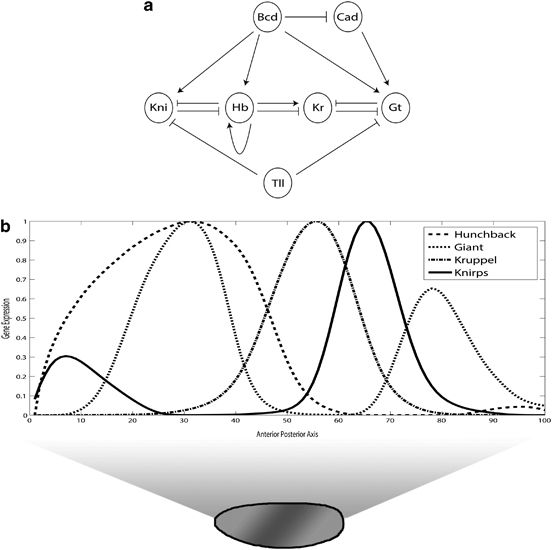
\includegraphics[scale=0.75]{tex/review/hdy201352f1.jpg}
    \caption{(a) Gene regulatory network for Drosophila gap genes, showing relationship between input genes (Bcd, Cad, Hb, Tll) and output genes (Kni,Hb,Kr,Gt). (After figure 1 of Papatsenko and Levine\cite{papatsenko11}). (b) Concentration of Gap genes along the anterior posterior axis of the embryo. Model was fitted to this data. Hb, hunchback; Gt, giant; Kr, Kruppel; Kni, Knirps.}
    \label{fig:review1}
\end{figure}

The Drosophila gap gene network provides early response to maternal gradients in the Dropsophila embryo segmentation pathway. The gap gene’s concentration is set up through cues from maternal genes and mutual repression between the gap genes. Using a modular approach, the gap genes can be divided into network domains, where each domain contains a toggle switch corresponding to a pair of gap genes. The toggle switches resemble the phage lambda bi-stable switch, except the gap genes concentrations are positionally operated through the maternal genes’ gradients with synthesis rates for competing components changing along the anterior–posterior (AP) axis.

Based on this principle, Papatsenko and Levine \cite{papatsenko11} developed a dynamic model for gap gene expression, which exploits elements of fractional site occupancy. The model accounts for diffusion of the gap genes along the AP axis through a system of differential equations and requires five to seven parameters to fit quantitative spatial expression data for gap gene expression gradient. In their paper, Papatsenko and Levine show how the model can account for large effect mutations in the network with a shift in gap gene concentration. The model is illustrated in fig. \ref{fig:review1}.

In this simple example, the network is sufficiently small that it can be solved numerically. Papatsenko and Levine therefore utilized a Metropolis optimization algorithm for fitting their model, where the objective function was based on a measure of correlation between the model and the data. Different fitting ranges were defined for the gap genes along with the length of the embryo.

Of course, such networks include a noise component, both in underlying gene expression and in error of measurement of those expression values. An optimization approach, such as that used in Papatsenko and Levine, will struggle to deal with this, but a fully Bayesian approach remains possible, as we demonstrate using a MCMC analysis. We present results for both a standard MCMC analysis and the ABC variant of MCMC. For a more detailed overview of both methods, see Marjoram and Tavare \cite{Marjoram2006}.

We show the results of such a Bayesian analysis, in terms of the resulting predictive power, in fig. \ref{fig:review2} . In the top row, we show the observed levels of expression (y axis) for each of the four measured genes at each of 100 points sampled along the AP axis of the embryo (x axis). Each gene corresponds to a single column of the figure: Hb, Gt, Kr and Kni (reading left to right). In rows two to four, we show the fits resulting from analyses of that data. In each row, the y axis represents the predicted expression levels. In row two, we show the results obtained by Papatsenko and Levine using a Metropolis optimization algorithm. We note that in that paper they chose to focus on a domain of interest in which the gene expression gradients were greatest, indicated by the region between the two vertical, dashed lines on the plots. In row three, we show results obtained by sampling a single set of parameter values from the posterior distribution resulting from an MCMC analysis of the entire length of the anterior– posterior axis. In row four, we show results obtained by sampling a single set of parameter values from the posterior distribution resulting from an ABC analysis of the entire length of the anterior–posterior axis.
\begin{figure}
    \centering
    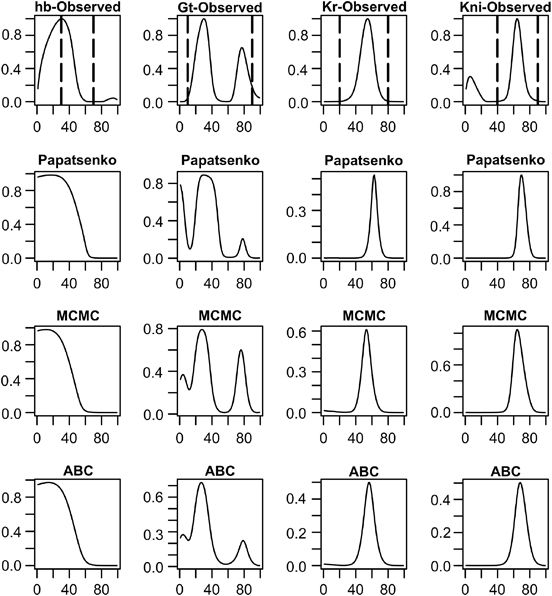
\includegraphics[scale=0.75]{tex/review/hdy201352f2.jpg}
    \caption{Predicted power of analysis of anterior–posterior gap genes for Drosophila. The x axis corresponds to the anterior–posterior axis of the embryo. The y axis indicates the observed (fitted) levels of gene expression in rows 1 (2–4). Top row: observed levels of expression for each of four measured genes: Hb, Gt, Kr and Kni (reading left to right). Row two: fits from Papatsenko and Levine optimization approach. Row three: results sampled from posterior of Bayesian Markov chain Monte Carlo method (MCMC) analysis. Row four: results sampled from posterior of approximate Bayesian computation (ABC) analysis. Vertical lines show the domain of interest of Papatsenko and Levine.}
    \label{fig:review2}
\end{figure}

The figure shows that both the MCMC and ABC analyses fit well. We note in passing that the fit resulting from both the MCMC and ABC analyses over the domain of interest is significantly better than that resulting from the analysis of Papatsenko and Levine, despite the fact that the former analyses fit over the entire length of the embryo. The benefit of the Bayesian approaches is that full posterior distributions are obtained for each of the parameters. As an illustration, we show the posterior distributions resulting from the MCMC analysis in fig. \ref{fig:review3}. We show posterior distributions for four parameters: the cooperativity, C, the synthesis/decay rate, alpha and node-specific binding affinities, K1 and K2. The ABC method typically results in slightly wider posterior distributions for parameters due to the increased tolerance allowed in the analysis. This will likely to be reflected in a reduction in predictive power (seen in fig. \ref{fig:review3}). Thus, it is important to stress that when exact calculation of likelihoods is possible, standard Bayesian approaches, such as MCMC, should be used. However, for more complex (and possibly, therefore, more realistic) networks, an exact MCMC analysis will be impossible, whereas the ABC approach will remain tractable.

\begin{figure}
    \centering
    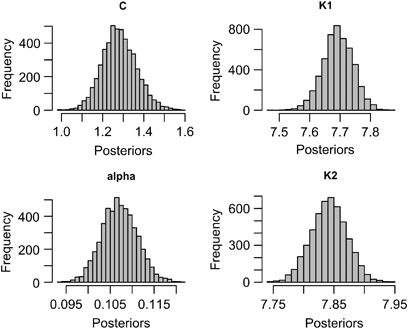
\includegraphics{tex/review/hdy201352f3.jpg}
    \caption{Posterior distributions from Markov chain Monte Carlo method analysis. Shown are distribution for cooperativity, C; synthesis/decay rate, alpha; and node-specific binding affinities, K1 and K2.}
    \label{fig:review3}
\end{figure}

\section{Conclusion}
We are in the middle of a golden age of genetics in which we are discovering unheralded numbers of polymorphisms that are (marginally) associated with phenotypic variance. Although the efforts so far represent a great leap forward, true understanding will only be obtained when we move from association to causation by building an integrated GP map. In doing so, we will not only increase analytic power of discovery, but also move a step closer to impacting human health, as well as animal and plant breeding, in more effective ways. At the same time, we note that stochastic elements that are likely to be present in many networks will mean that complete predictability will never be attained (a statement that is also likely to be true for systems that lack genuine stochasticity, but which are highly complex and will likely therefore never be fully characterized).

In this chapter, we have considered what we have learned so far from the recent flood of GWAS and other data, and in what directions that evidence suggests we should next turn. We do not intend this review as an opinion piece regarding whether GWAS should be labeled as a success or otherwise. We regard this argument to be one of semantics more than content. GWAS has found a large number of polymorphisms associated with phenotype, and will continue to do so. However, it is equally clear that much heritability remains unexplained. Our belief is that now that we have determined what percentage of heritable variation can be explained by polymorphism using marginal statistical analysis (and often using relatively common polymorphism), we face a fork in the road in which one path is labeled `more data', whereas the other is labeled `more biology'. Although both paths are clearly useful, we believe there is much to be gained by considering the latter fork and exploiting the ability of biological knowledge to inform statistical analysis as we attempt to move from association to function, and it is on this perspective that we have focused in this chapter.

Here, our focus has been upon incorporating biological insight via explicit modeling of underlying pathways. However, we also note that there is a growing trend to incorporate biological information into the prior distribution when searching large numbers of SNPs for association with phenotype. For example, one can take information from annotation databases such as \href{http://www. pantherdb.org/}{PANTHER}. This can be viewed as a way of increasing power in the face of increasing multiple comparison penalties.

An advantage of a fully Bayesian analysis of pathways, such as we have proposed here, is that the sensitivity to a given parameter is fully described in the resulting parameter posterior distribution. Given this, we envision the following flow of analysis. Using a Bayesian analysis for each genotype, the parameters important for GRN function are determined. A combination of whole-organism and GRN-specific molecular phenotypes is used. We then infer which GRN perturbation results in which whole-organism phentotype. The relative sensitivities of the phenotypes to perturbations in different GRN nodes and paths are evaluated to select the best targets for disease treatment. When a perturbation of the parameter is detected in a certain genotype, a localized search for the polymorphisms affecting this parameter is made using GWAS-like approaches, focused on specific nodes and/or paths in the GRN. The analyses among genotypes sharing that polymorpshism are then merged to more precisely characterize the effect of the polymorphism on the GRN behavior, much as in a regular GWAS.

This combination of GRN and GWAS approaches will ultimately enable collapsing of the effects of multiple polymorphisms - including those of low frequency—into larger groups of `shared' functional effect. The GRN state, and the effects of groups of functionally similar polymorphisms on that state, could then be compared between individuals experiencing different environments, or between those who are healthy and those who exhibit disease.

Finally, we note that analysis of GRNs such as those we have described here can be extremely computationally intensive, particularly for a method such as ABC. However, ABC approaches also provide several avenues for optimization. In particular, ABC demands repeated simulation from models, and the number of repeats is likely to be very large—the more simulations we perform, the greater the level of agreement between observed and simulated data that can be insisted upon, and therefore the greater (typically) the level of accuracy that can be obtained. It is therefore possible to `parallelize' algorithms and run them over multiple computational nodes, rather than have one node independently simulate data over and over again. N nodes will decrease the analysis time by roughly a factor of N, compared with a single node. This can be achieved on computational ‘clusters’ or, perhaps more cost effectively, by exploiting Graphical Processing Units, which provide extreme increases in computational efficiency when the repeated unit (here the simulation) is relatively straightforward.

In conclusion, we are in the midst of a golden era of genomics, offering the potential to move from association to causation. However, the success of GWAS is likely to be limited by a number of factors. In this chapter, we have discussed some of those factors and offered a possible paradigm for moving forwards form this point in a way that addresses some of those limitations.